\documentclass{article} % \documentclass{} is the first command in any LaTeX code.  It is used to define what kind of document you are creating such as an article or a book, and begins the document preamble

\usepackage{amsmath} % \usepackage is a command that allows you to add functionality to your LaTeX code
\usepackage{graphicx}
\graphicspath{ {./images/} }
\title{Discrete Time Signals and Systems} % Sets article title
\author{Hunter Mills} % Sets authors name
\date{\today} % Sets date for date compiled

% The preamble ends with the command \begin{document}
\begin{document} % All begin commands must be paired with an end command somewhere
    \maketitle % creates title using information in preamble (title, author, date)
    
    \section{Frequency Analysis of Signals} % creates a section
    Two of the most important mathematical tools in engineering is the Fourier Transform and Fourier Series. In this chapter they will be used to do frequency analysis. This signal representations basically involve the decomposition of the signals into terms of sinusoidal functions. For infinite periodic signals, use the Fourier series and for a finite energy series use the Fourier transform. These decomposition are very important in LTI systems since the response of an LTI signal to a sinusoid is a sinusoid of the same frequency but different amplitude and phase.
    \subsection{Euler's Identity}
    \begin{equation}
 	e^{j\theta} = \cos(\theta) + j\sin(\theta)
	\end{equation}
	\begin{equation}
 	\cos(\theta) = \frac{e^{j\theta} + e^{-j\theta}}{2}
	\end{equation}
	\begin{equation}
 	\sin(\theta) = \frac{e^{j\theta} - e^{-j\theta}}{j2}
	\end{equation}
	\begin{equation}
 	\cos(\Omega_k t) = \frac{1}{2}(e^{j\Omega_k t} + e^{-j\Omega_k t})
	\end{equation}
	\begin{equation}
 	\sin(\Omega_k t) = \frac{-j}{2}(e^{j\Omega_k t} - e^{-j\Omega_k t})
	\end{equation}
    
    \subsection{Frequency Analysis of Continuous Time Signals}
    \textbf{The Fourier Series for CT Periodic Signals}
    
    The Fourier Series is a representation of the signal as a linear weighted sum of harmonically related sinusiods or complex exponentials. From chapter 1, we can recall that a linear combination of harmonically related complex exponentials of the form
    \begin{equation}
 	x(t) = \sum_{k=-\infty}^{\infty}c_ke^{j2\pi kF_0t}     
	\end{equation}
	is a periodic signal with fundamental period $T_P = 1/F_0$. Hence we can think of the exponential signals
	\begin{equation}
 	 {e^{j2\pi kF_0t}, \;\;\;\;\;\; k = 0, \pm 1, \pm 2 ...}
	\end{equation}
	as the building blocks to construct periodic signals by the proper choice of fundamental frequency and $c_k$. The Fourier series coefficients can be calculated with:
	\begin{equation}
 	c_k = \frac{1}{T_P} \int_{T_P} x(t)e^{-j2 \pi kF_0t}dt.
	\end{equation}
	In general the Fourier coefficients $c_k$ are complex. It is easily shown that if the periodic signal is real, $c_k$ and $c_{-k}$ are complex conjugates. As a result:
	\begin{equation}
 	c_k = |c_k|e^{j\theta_{k}}
	\end{equation}
	then
	\begin{equation}
 	c_{-k} = |c_k|^{-j\theta_{k}}
	\end{equation}
	Consequently the FS can be represented as:
	\begin{equation}
 	x(t) = c_0 + 2\sum_{k=1}^{\infty}|c_k|\cos(2\pi k F_0t + \theta_{k})    
	\end{equation}
	or 
	\begin{equation}
 	Trigonometric: x(t) = a_0 + \sum_{k=1}^{\infty}(a_k\cos(2\pi kF_0t) - b_k\sin(2\pi kF_0t))
	\end{equation}
	\begin{equation}
 	Harmonic: x(t) = A_{DC} + \sum_{k=1}^{\infty}\sqrt{a_k^2+b_k^2} \cos(\Omega_{k}t - \theta_{k}) 
	\end{equation}
	where $a_0 = c_0$, $a_k = 2|c_k|\cos(\theta_{k})$, and $b_k = 2|c_k|\sin(\theta_{k})$. These are called the \textit{Continuous Time
	Fourier Series} (CTFS).\\
	\\
	The Dirichlet conditions guarantee convergence and the series converges to x(t) when\\
	\textbf{1.} Signal has a finite number of discontinuities in any period.\\
	\textbf{2.} Signal has a finite maxima and minima in any period.\\
	\textbf{3.} Signal is absolutely summable. \\
	\\
	\textbf{Power Density Spectrum of Periodic Signals}\\
	
	A periodic signal has infinite energy and a fine average power. Using the FS the \textbf{Parsevals Relation for Power Signals} becomes clear.
	\begin{equation}
 	P_x = \frac{1}{T_P} \int_{T_P} |x(t)|^2dt = \sum_{k=-\infty}^{\infty} |c_k|^2
	\end{equation}
	If we would plot $|c_k|^2$ as a function of the frequencies $kF_0, k=0,\pm 1, \pm 2,...$ then figure 1 shows the \textit{power density spectrum}.
	
	\begin{figure}[h]
    \centering
	\includegraphics[width=10cm]{pds}
	\caption{Power Density Spectrum}
	\end{figure}
	
	This is called a line spectrum and the spacing between the spectral lines is the fundamental frequency. The total average power can be expressed as 
	\begin{equation}
 	P_x = c_0^2 + 2\sum_{k=1}^{\infty}|c_k|^2
	\end{equation}
	\begin{equation}
 	P_x = a_0^2 + \frac{1}{2}\sum_{k=1}^{\infty}(a_k^2 + b_k^2)
	\end{equation}
	\\
	\\
	\textbf{The Fourier Transform for CT Aperiodic Signals}\\
	As the period of a wave increases towards infinity, the spacing between the line spectrum decreases towards zero. When the period becomes
	infinite the spacing becomes zero and the spectrum is continuous. Consider the aperiodic and finite signal x(t)
	\begin{equation}
	x(t) = \lim_{T_P \rightarrow \infty}x_P(t).
	\end{equation}
	This implies that we should be able to get the spectrum for x(t) from the spectrum of $x_P(t)$ and by taking the limit as $T_P \rightarrow \infty$.
	The \textbf{CT Fourier Transform} is defined as
	\begin{equation}
	X(F) = \int_{-\infty}^{\infty}x(t)e^{-j2\pi Ft}dt.
	\end{equation}
	A relationship between the Fourier transform and the Fourier series is
	\begin{equation}
	T_Pc_k = X(kF_0) = X(\frac{k}{T_P})
	\end{equation}
	The inverse Fourier Transform is defined as 
	\begin{equation}
	x(t) = \int_{-\infty}^{\infty}X(F)e^{j2\pi Ft}dF.
	\end{equation}	
	This is called the \textit{Continuous Time Fourier Transform} (CTFT). The difference between the Fourier transform and series 
	the former is continuous and hence the synthesis of an aperiodic signal
	from its spectrum is done by integration not summation. The previous Fourier transform equations can also be represented
	with its radial frequency, $\Omega$.
	\begin{equation}
	x(t) = \frac{1}{2\pi}\int_{-\infty}^{\infty}X(\Omega)e^{j\Omega t}d \Omega.
	\end{equation}
	\begin{equation}
	x(\Omega) = \int_{-\infty}^{\infty}x(t)e^{j\Omega t}dt.
	\end{equation}
	\\
	\\
	\textbf{Dirichlet Condition for Fourier Transform to exist}\\
	\textbf{1.} x(t) must have at most a finite number of finite discontinuities\\
	\textbf{2.} x(t) must have at most a finite number of maxima and minima\\
	\textbf{3.} x(t) is absolutely integral that is $\int_{-\infty}^{\infty}|x(t)|^2dt < \infty$\\
	\\
	\\
	\textbf{Energy Density Spectrum of Aperiodic Signals}\\
	Let x(t) be any finite energy signal, its energy is
	\begin{equation}
	E_x = \int_{-\infty}^{\infty}|x(t)|^2dt.
	\end{equation}
	Parsevals relation for finite energy signals is:
	\begin{equation}
	E_x = \int_{-\infty}^{\infty}|x(t)|^2dt = \int_{-\infty}^{\infty}|X(F)|^2dF
	\end{equation}
	and it expresses the principle of conservation of energy in the frequency and time domain. The energy in a signal over a frequency 
	band is,
	\begin{equation}
	E = \int_{F_1}^{F_1+\Delta F}|X(F)|^2dF
	\end{equation}
	If the signal x(t) is real then 
	\begin{equation}
	|X(-F)| = |X(F)|
	\end{equation}
	\begin{equation}
	\angle X(-F) = -\angle X(F)
	\end{equation}

	\subsection{Frequency Analysis if DT Signals}
	In contrast to CT signals which $-\infty < f < \infty$ the frequency range for DT signals is $(-\pi , \pi)$ or $(0, 2\pi)$. A DT signal of
	fundamental period N can consist of frequency components separated by $2\pi /N$ radians or $f = 1/N$ cycles. Consequently,
	the Fourier series representation will contain at most N frequency components. \\
	\textbf{The Fourier Series for DT periodic signals}\\
	Suppose we have x(n) with period N. The Fourier series representation for x(n) consists of N harmonically related exponential functions,
	\begin{equation}
	e^{j2\pi kn/N}, \;\;\;\;\; k = 0,1, ..., N-1
	\end{equation}
	and is expressed as
	\begin{equation}
	x(n) = \sum_{k=0}^{N-1}c_ke^{j2\pi kn/N}
	\end{equation}
	where 
	\begin{equation}
	c_k = \frac{1}{N}\sum_{n=0}^{N-1}x(n)e^{-j2\pi kn/N}
	\end{equation}
	This is called the \textit{Discrete Time Fourier Series} (DTFS). $c_k$ provide the description of x(n) in the frequency domain
	in the sense that $c_k$ represents the amplitude and phase associated with the frequency component
	\begin{equation}
	s_k(n) = e^{j2\pi kn/N} = e^{j\omega_k n}
	\end{equation}
	where $\omega_k = 2\pi k/N$. The spectrum of a singal x(n), which is periodic N, is a periodic sequence with period N, ie the 
	spectrum repeats.
	\\
	\\
	\textbf{Power Density Spectrum of Periodic Signals}\\
	The average power of a DT periodic signal with period N is
	\begin{equation}
	P_x = \frac{1}{N}\sum_{n=0}^{N-1}|x(n)|^2.
	\end{equation}
	Using the Fourier series coefficients we can calculate the power using Parseval's relation for DT periodic signals.
	\begin{equation}
	P_x = \sum_{k=0}^{N-1}|c_k|^2
	\end{equation}
	To get the energy in a period multiply the power by N. Since the spectrum is periodic about N, the magnitude and phase properties are shown
	in the next figure.

	\begin{figure}[h]
	\centering
	\includegraphics[width=10cm]{sym}
	\caption{Magnitude and Phase Properties of DTFS}
	\end{figure}

	Other ways to calculate the DTFS is with
	\begin{equation}
	x(n) = c_0 + 2\sum_{k=1}^{L}|c_k|\cos (\frac{2\pi}{N}kn + \theta_k)
	\end{equation}
	or 
	\begin{equation}
	x(n) = a_0 + \sum_{k=1}^{L}(a_k \cos(\frac{2\pi}{N}kn)- b_k \sin(\frac{2\pi}{N}kn))
	\end{equation}
	where $a_0 = c_0, a_k = 2|c_k|\cos \theta_k, b_k = 2|c_k|\sin \theta_k and L = N/2$ if N is even and $L = (N-1)/2$ if odd.\\
	\textbf{The Fourier Transform of DT Aperiodic Signals}\\
	This section heavily parallels the section for CTFT. The Discrete Time Fourier Transform (DTFT) is defined as
	\begin{equation}
	X(\omega) = \sum_{n = -\infty}^{\infty}x(n)e^{-j\omega n}
	\end{equation}
	The same as the CTFS and DTFS, the DTFT has a frequency range over $(0, 2\pi)$ and is periodic with $2\pi$
	To go from the frequency domain to the time domain, the inverse Fourier transform is
	\begin{equation}
	x(n) = \frac{1}{2\pi}\int_{-\pi}^{\pi}X(\omega)e^{j\omega n}d\omega
	\end{equation}
	\textbf{Convergence of the Fourier Transform}\\

	If the value $\sum_{n=-\infty}^{\infty}|x(n)| < \infty$ then this condition (absolutely summable) is sufficient for the existence of the DTFT. Some
	signals are not absolutely summable but they are square summable ($E_x = \sum_{n=-\infty}^{infty}|x(n)|^2 < \infty$). If the signal is
	absolutely summable there will be \textit{uniform convergence}. If it is square summable then there will be \textit{mean-square convergence}
	where at jump discontinuities the DTFT converges to a midpoint and demonstrates Gibbs Phenomenon.
	\begin{figure}[h]
	\centering
	\includegraphics[width=5cm]{gibbs}
	\caption{DTFT and Gibbs Phenomenon}
	\end{figure}
	\textbf{Energy Density Spectrum of Aperiodic Signals}

	The energy in a DT signal x(n) is 
	\begin{equation}
	E_x = \sum_{n = -\infty}^{\infty}|x(n)|^2
	\end{equation}
	Using \textit{Parsevals relation for DT aperiodic signals} the energy can be calculated with
	\begin{equation}
	E_x = \int_{-\infty}^{\infty}|X(\omega)|^2d\omega
	\end{equation}
	If x(n) is real, the magnitude has even symmetry and the phase has odd. The symmetry properties let us calculated the magnitude and phase
	from the spectrum in the range $(0, \pi)$. \\
	\textbf{Frequency domain classification of Signals: Bandwidth}

	If the frequency components are located around zero Hz then the signal is considered baseband and low-frequency. The two types of signals
	are shown in the next figure. 

	\begin{figure}[h]
	\centering
	\includegraphics[width=5cm]{band}
	\caption{a: Baseband, b: High, c: Bandpass}
	\end{figure}
	The relative measurement of how wide the frequency components are is called the \textit{Bandwidth}. A narrowband signal is one
	where the bandwidth is much smaller (near 10x) than the median frequency otherwise it is wideband. A signal is bandlimited if its spectrum is zero outside
	the frequency band. 
	\begin{equation}
	|X(\Omega)| = 0 \;\; for \;\;|F| > B (Bandwidth)
	\end{equation}
	Without proving, no signal can be time-limited and bandlimited at the same time. A reciprocal relationship exists between the time 
	duration and the frequency duration. 

	\subsection{Frequency Domain and Time Domain Signal Properties}
	In the previous section we introduced 4 frequency analysis tools,\\
	\textbf{1.} The CTFS for periodic signals\\
	\textbf{2.} The CTFT for aperiodic signals\\
	\textbf{3.} The DTFS for periodic signals\\
	\textbf{4.} The DTFT for aperiodic signals\\
	Some other properties that can be derived are, CT signals have aperiodic spectra, DT signals have periodic spectra with 2$pi$, 
	periodic signals have discrete spectra (the FS is used which results in line spectra) and aperiodic finite energy signals have 
	continuous spectra. The following figure shows the summary of analysis and synthesis formulas. 
	\begin{figure}[h]
	\centering
	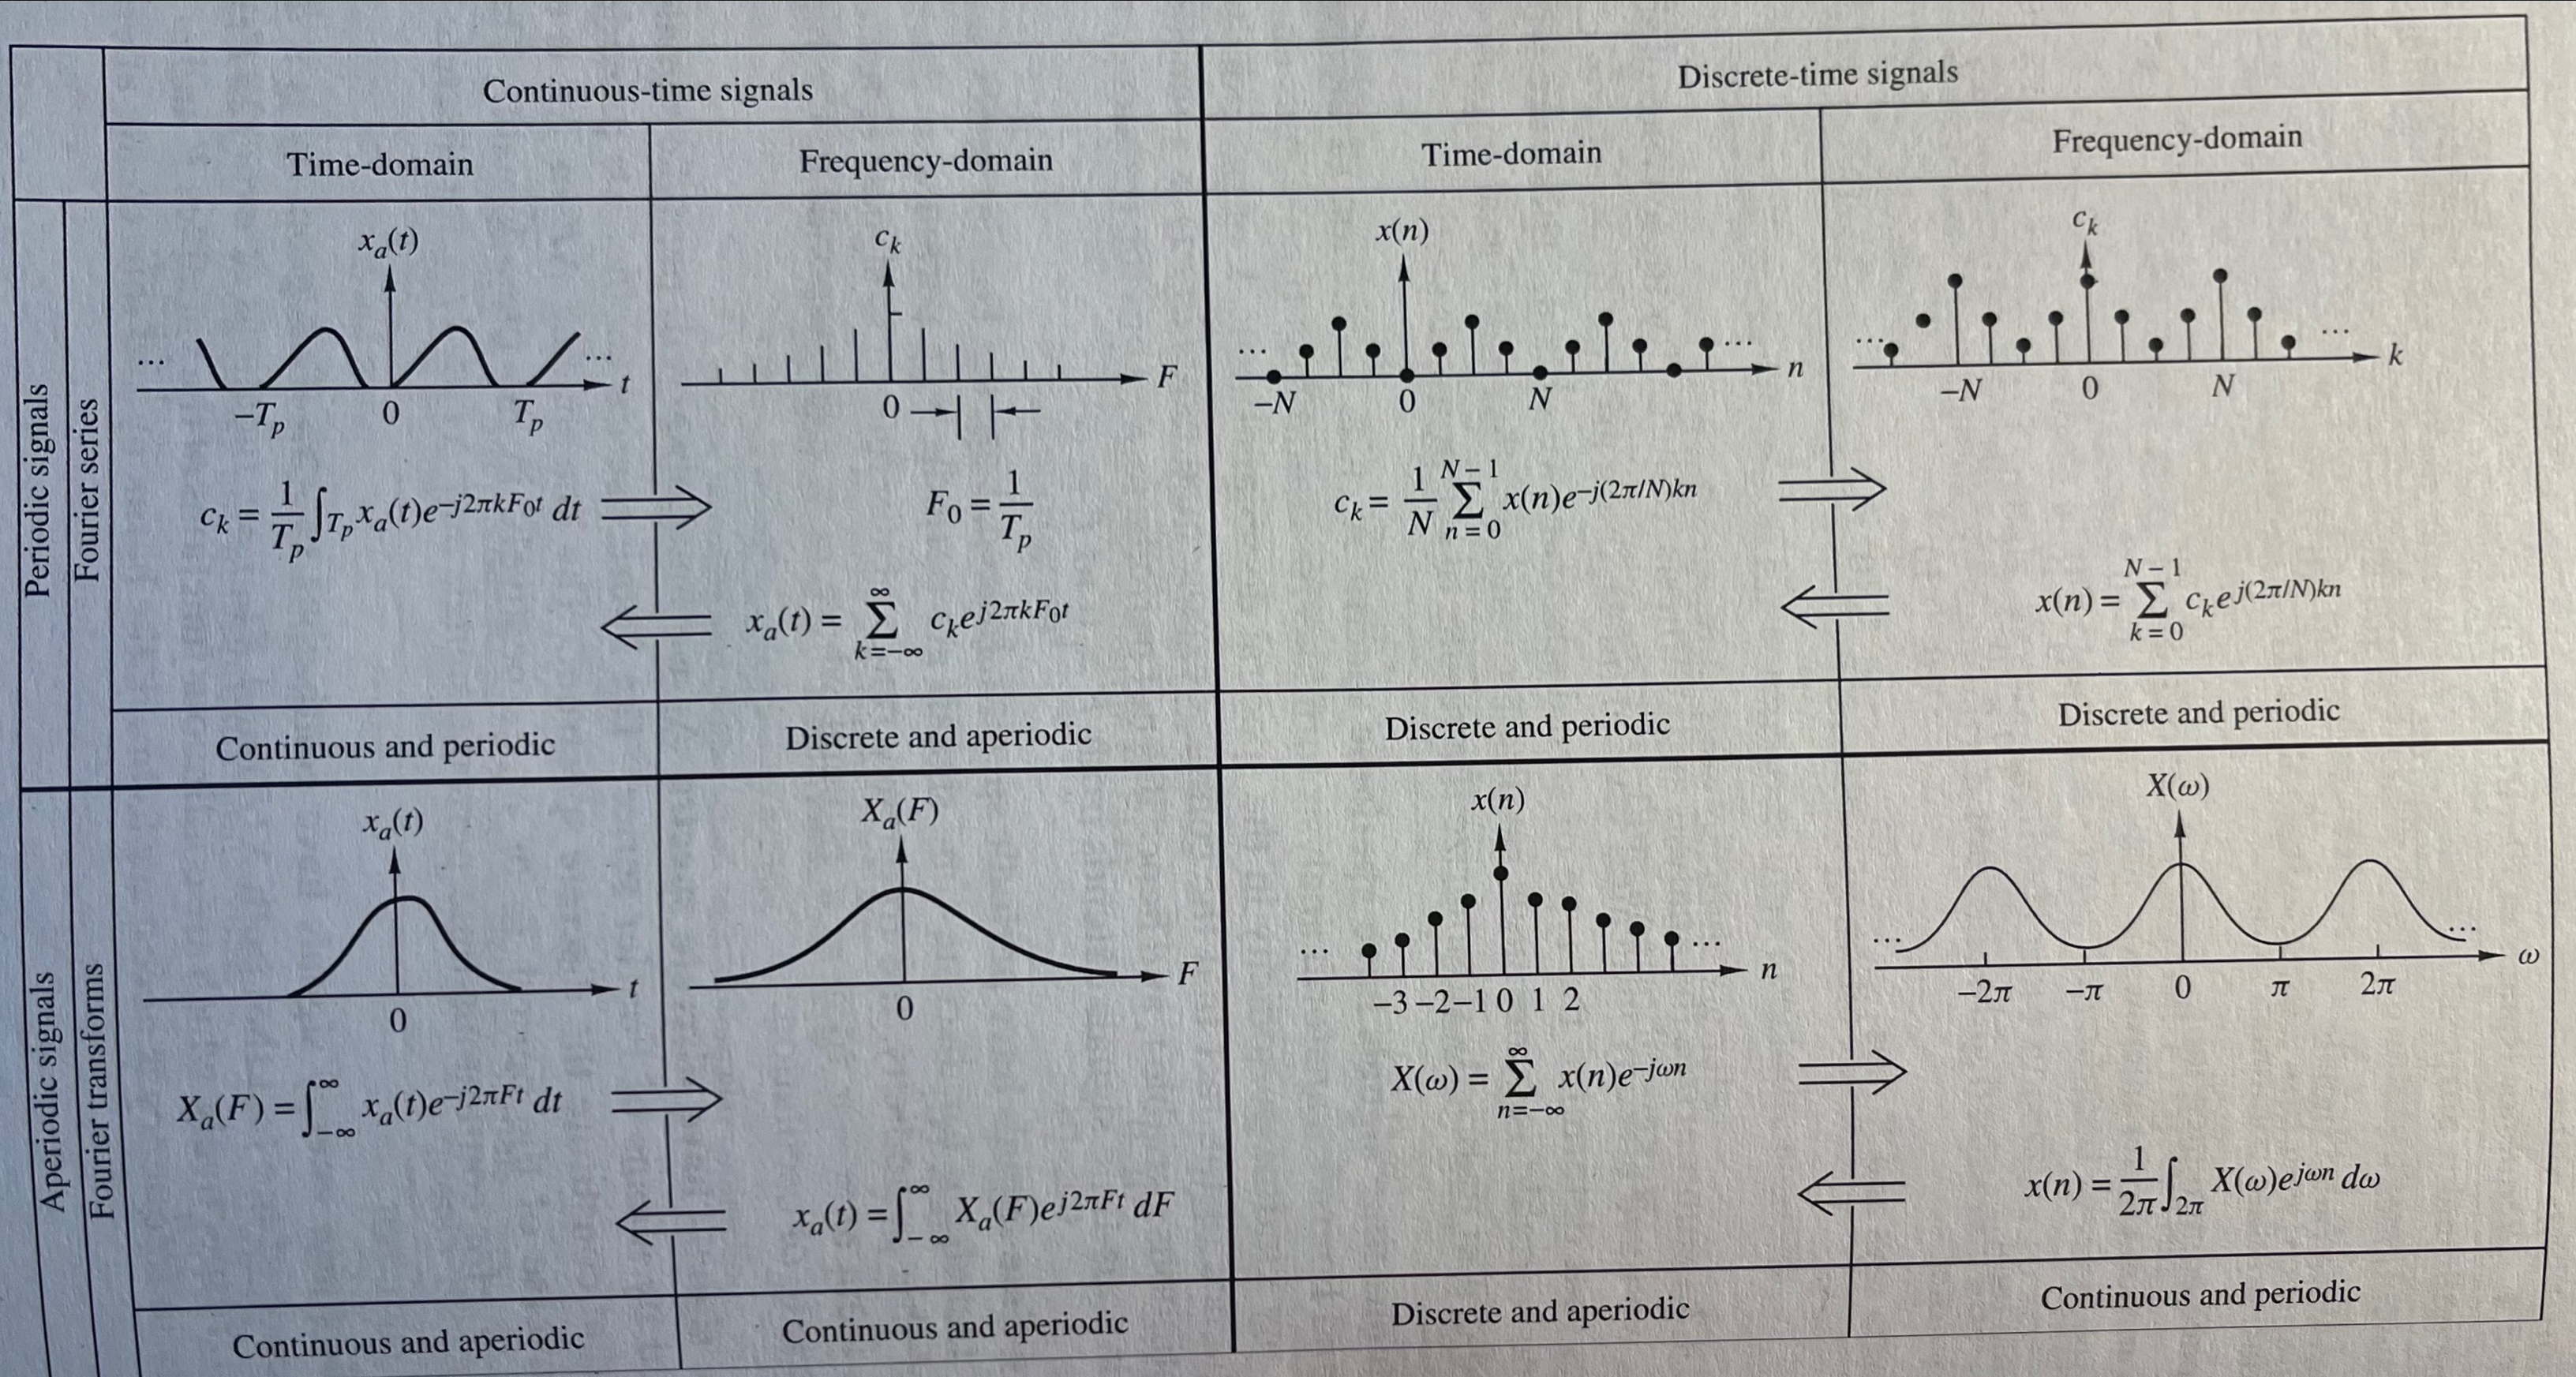
\includegraphics[width=12cm]{summary}
	\caption{Summary of analysis and synthesis equations}
	\end{figure}

	\subsection{Properties of the Fourier Transform for DT signals}
	The Fourier Transform for aperiodic finite-energy signals has a number of properties that can make the complexity of frequency
	analysis easier. $x(n) and X(\omega)$ are called Fourier transform pairs. In this section, I will not derive the properties, but
	there will be diagrams. \\
	\textbf{Symmetry Properties of the Fourier Transform}\\
	When a signal satisfies some symmetry properties in the time domain, these properties impose some symmetry conditions in the frequency
	domain.\\
	\textbf{Real Signals}\\
	When x(n) is a real signal, the magnitude and phase spectra possess the following symmetry properties
	\begin{equation}
	|X(\omega)| = |X(-\omega)| \; (even)
	\end{equation}
	\begin{equation}
	\angle X(-\omega) = - \angle X(\omega) \;(odd)
	\end{equation}
	\textbf{Real and Even Signals}
	\begin{equation}
	X(\omega) = X_R(\omega) = x(0) + 2\sum_{n=1}^{\infty}x(n) \cos(\omega n)
	\end{equation} 
	If the input x(n) is real and even then the spectra will be real-valued.\\
	\textbf{Real and Odd Signals}
	\begin{equation}
	X(\omega) = X_I(\omega) = -2\sum_{n=1}^{\infty}x(n) \sin(\omega n), 
	\end{equation}
	thus real and odd signals produce a purely imaginary spectrum. 
	\begin{figure}[h]
	\centering
	\includegraphics[width=10cm]{real}
	\caption{Real Signal FT Properties}
	\end{figure}

	\begin{figure}[h]
	\centering
	\includegraphics[width=10cm]{symm}
	\caption{Symmetry Diagram}
	\end{figure}
	\textbf{Fourier Transform Theorems and Properties}\\
	All of these properties are summed up well in the following table.
	\begin{figure}[h]
	\centering
	\includegraphics[width=10cm]{prop}
	\caption{FT Properties}
	\end{figure}
	In Parsevals relation, when $x_1(n) = x_2(n) = x(n)$ then
	\begin{equation}
	\sum_{n=-\infty}^{\infty}|x(n)|^2 = \frac{1}{2\pi}\int_{2\pi}|X(\omega)|^2
	\end{equation}








\end{document} % This is the end of the document